%%%%%%%%%%%%%%%%%%%%%%%%%%%%%%%%%%%%%%%%%%
% CHAPTER 1 Essential Concepts
%%%%%%%%%%%%%%%%%%%%%%%%%%%%%%%%%%%%%%%%%%

\chapter{Essential Concepts}

\section{Functions}
\marginnote{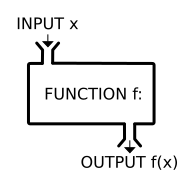
\includegraphics[scale=0.8]{pics/schematic}}
\begin{mybox}{Definition of a function}
	A functioon $f $ from a set $X $ to a set $Y $ is an assignment of one element of $Y$ to each element of $X$, where
	\begin{itemize}
		\item The set $X$ is called the \emph{domain} of the function.
		\item The set $Y$ is called the \emph{codomain} of the function.
	\item Notation: $f: X \rightarrow Y$ or $X {\overset{f}{\to}} Y$ or $x\mapsto f(x)$
	\end{itemize}
\end{mybox}
\marginnote{

\includegraphics[scale=0.8]{pics/multivariate}
A multivariate function $f: U \rightarrow f(x_{1},\ldots,x_{n})$, where $x_{1} \in X_{1}, \ldots, x_{n} \in X_{n}$, the domain $U$ has the form $U \subseteq X_{1} \times \ldots \times X_{n}$, $X_{1} \times \ldots \times X_{n}$ is the Cartesian product of $X_{1}, \ldots, X_{n}$
}
\begin{examplebox}{(Probability density functions and likelihood functions)}
	Identify the independent variables of the following functions:

	\[
		f(x) = \frac{1 }{\sqrt{2 \pi \sigma^{2}}}e^{-\frac{(x-\mu)^{2}}{2 \sigma^{2}}}
	\]

	\[
P(y_{i }) = \frac{1 }{\sqrt{2 \pi \sigma^{2}}} e^{- \frac{1 }{2 \sigma^{2 }}(y_{i }-\alpha-\beta x_{i } - \gamma x_{i }^{2})^{2}}
	\]

	\begin{align*}
	L(\alpha,\beta,\gamma,\sigma^{2}) &= \prod^{n}_{i=1}P(y_{i })
	&=\left(\frac{1 }{\sqrt{2 \pi  \sigma^{2}}}\right)^{n} e^{- \frac{1 }{2 \sigma^{2 }} \sum^{n }_{i=1}(y_{i }-\alpha-\beta x_{i } - \gamma x_{i }^{2})^{2}}
	\end{align*}

\end{examplebox}

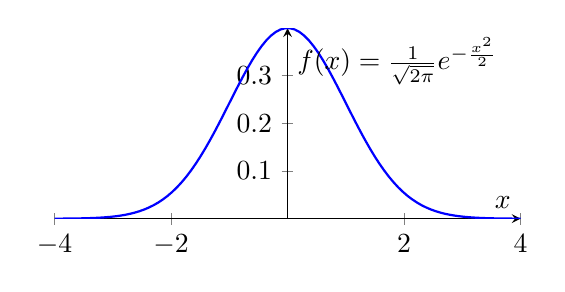
\begin{tikzpicture}
	\begin{axis}[
		axis lines = middle,
		xlabel = \(x\),
	ylabel = {\(f(x) = \frac{1}{\sqrt{2\pi}}e^{-\frac{x^{2}}{2}}\)},
		domain=-4:4,
		samples=100,
		width=7.5cm,
		height=4cm,
		ymajorgrids=false,
		xmajorgrids=false,
	]
	\addplot [
		thick,
		blue,
	] {1/sqrt(2*pi) * exp(-x^2/2)};
	\end{axis}
\end{tikzpicture}

\section{Common types of functions}

\marginnote{
	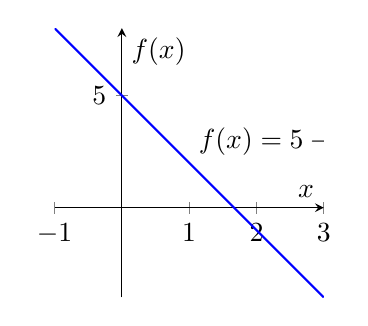
\begin{tikzpicture}
    \begin{axis}[
        axis lines = middle,
        xlabel = \(x\),
        ylabel = {\(f(x)\)},
        domain=-1:3,
        samples=100,
        width=5cm,
        height=5cm,
        ymajorgrids=false,
        xmajorgrids=false,
    ]
    \addplot [
        thick,
        blue,
    ] {5 - 3*x };
		\node at (axis cs:1, 4) [anchor=north west] {\(f(x) = 5 - 3x\)};
    \end{axis}
\end{tikzpicture}

\vspace{1cm}

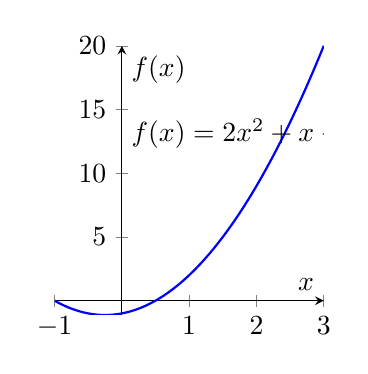
\begin{tikzpicture}
    \begin{axis}[
        axis lines = middle,
        xlabel = \(x\),
        ylabel = {\(f(x)\)},
        domain=-1:3,
        samples=100,
        width=5cm,
        height=5cm,
        ymajorgrids=false,
        xmajorgrids=false,
    ]
    \addplot [
        thick,
        blue,
    %] {-x^2 +2*x+1};
    ] {2*x^2 +x-1};
    % Add the function expression
    \node at (axis cs:0, 15) [anchor=north west] {\(f(x) = 2x^2 +x-1\)};
    \end{axis}
\end{tikzpicture}

\vspace{1cm}

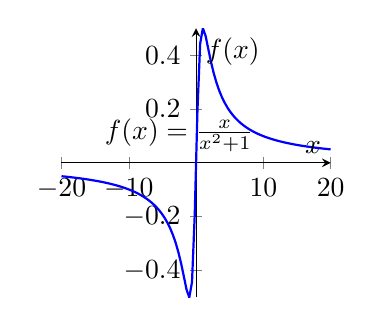
\begin{tikzpicture}
    \begin{axis}[
        axis lines = middle,
        xlabel = \(x\),
        ylabel = {\(f(x)\)},
        domain=-20:20,
        samples=100,
        width=5cm,
        height=5cm,
        ymajorgrids=false,
        xmajorgrids=false,
    ]
    \addplot [
        thick,
        blue,
    %] {-x^2 +2*x+1};
    ] {x / (x^2+1)};
    % Add the function expression
		\node at (axis cs:-15, 0.2) [anchor=north west] {\(f(x) = \frac{x}{x^{2}+1}\)};
    \end{axis}
\end{tikzpicture}
\vspace{1cm}

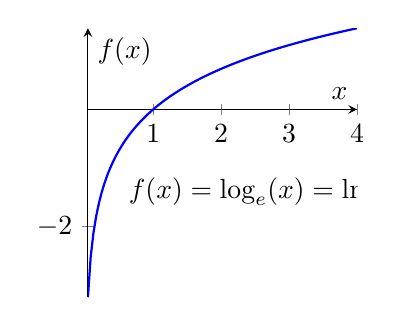
\begin{tikzpicture}
    \begin{axis}[
        axis lines = middle,
        xlabel = \(x\),
        ylabel = {\(f(x)\)},
        domain=0:4,
        samples=100,
        width=5cm,
        height=5cm,
        ymajorgrids=false,
        xmajorgrids=false,
    ]
    \addplot [
        thick,
        blue,
    %] {-x^2 +2*x+1};
    ] {ln(x)};
    % Add the function expression
    \node at (axis cs:0.5, -1) [anchor=north west] {\(f(x) = \log_e(x) = \ln(x), \quad x>0\)};
    \end{axis}
\end{tikzpicture}
}
\marginnote{
	* $e = \lim_{n \to \infty}(1+\frac{1}{n})^{n}$ or $e = \sum^{\infty}_{n=0} \frac{1}{n!}$
}
\begin{mybox}{Common types of functions}

\begin{itemize}
	\item \emph{Linear Functions:} Represented by $f(x)=ax+b$, where $a$ and $b$ are constants. The graph is a straight line.
	\item \emph{Quadratic Functions:} Represented by $f(x)=ax^{2}+bx+c$, where $a$, $b$, and $c$ are constants. The graph is a parabola.
	\item \emph{Polynomial Functions:} Represented by $f(x) = a_{n }x^{n }+a_{n-1 }x^{n-1 }+\ldots+a_{1 }x + a_{0}$, where $a_{n }, a_{n-1 }, \ldots, a_{1 }, a_{0 }$ are constants and $n$ is a non-negative integer. The graph varies depending on the degree $n$.
	\item \emph{Rational Functions:} Represented by $f(x) = \frac{P(x)}{Q(x)}$, where $P(x)$ and $Q(x)$ are polynomial functions and $Q(x)\neq0$. The graph can have vertical and horizontal asymptotes.
	\item \emph{Exponential Functions:} Represented by $f(x) = a \cdot b^{x}$, where $a $ and $b $ are constants and $b>0$. The graph increases (if $b>1$) or decreases (if $0<b<1$)
	\item \emph{Logarithmic Functions:} Represented by $f(x) = a \cdot \log_{b}(x) + c, \quad x>0$, where $a, b$, and $c$ are constants and $b > 0$. The graph is the inversse of an exponential function. When $a=1, b=e=2.718281828459, c=0$, $f$ is called the \emph{natural logrithm} of $x$, denoted as $ f(x) = \ln(x)$, the graph is strictly increasing on its domain.
	\item ...
\end{itemize}

\end{mybox}

\section{Limits}

A limit describes the value that a function (or sequence) approaches as the input (or index) approaches some value. Limits are fundamental to calculus and mathematical analysis and are used to define concepts like continuity, derivatives, and integrals.

%\subsection{Understanding Limits:}

\begin{mybox}{Definition}
The limit of $f(x)$ as $x$ approaches $c$ is $L$, denoted as $\lim_{x \to c}f(x)=L$, if for every number $\epsilon > 0$, there exists a number $\delta > 0$ such that $0<|x-c|<\delta$ implies $|f(x)-L| < \epsilon$.
\end{mybox}

Intuitive Understanding: As $x$ gets closer and closer to $c$ from both sides, $f(x)$ gets closer and closer to $L$. The value of the limit is what $f(x)$ approaches, not necessarily what $f(x)$ equals when $x=c$.

%\subsection{Understanding continuity}

\section{Derivatives}

\marginnote{
	\emph{Basic Differentiation Rules:}
	\begin{itemize}
		\item Power Rule:
\[
\frac{d}{dx} [x^n] = nx^{n-1}
\]
Example: If \( f(x) = x^3 \), then
\[
f'(x) = 3x^2
\]
		\item Product Rule:
\[
\frac{d}{dx} [u(x) v(x)] = u'(x) v(x) + u(x) v'(x)
\]
Example: If \( f(x) = x^2 \sin(x) \), then
\[
f'(x) = 2x \sin(x) + x^2 \cos(x)
\]
		\item Quotient Rule:
\[
\frac{d}{dx} \left[ \frac{u(x)}{v(x)} \right] = \frac{u'(x) v(x) - u(x) v'(x)}{[v(x)]^2}
\]
Example: If \( f(x) = \frac{x}{\sin(x)} \), then
\[
f'(x) = \frac{\sin(x) - x \cos(x)}{\sin^2(x)}
\]
		\item Chain Rule:
\[
\frac{d}{dx} [g(h(x))] = g'(h(x)) h'(x)
\]
Example: If \( f(x) = \sin(x^2) \), then
\[
f'(x) = \cos(x^2) \cdot 2x
\]
	\end{itemize}
\vspace{1cm}
\emph{Common Derivatives:}
\begin{align*}
[c]' &= 0\\
[e^x]' &= e^x\\
[a^x]'  &= a^x \ln(a)\\
[\ln(x)]' &= \frac{1}{x}\\
[\log_a(x)]' &= \frac{1}{x \ln(a)}\\
[\sin(x)]' &= \cos(x)\\
[\cos(x)]' &= -\sin(x)\\
[\tan(x)]' &= \sec^2(x)\\
[\sin^{-1}(x)]' &= \frac{1}{\sqrt{1 - x^2}}\\
[\cos^{-1}(x)]' &= -\frac{1}{\sqrt{1 - x^2}}\\
[\tan^{-1}(x)]' &= \frac{1}{1 + x^2}
\end{align*}
}
A derivative represents the rate of change of a function with respect to a variable. It is the slope of the function's graph at any given point and indicates how the function's value changes as the input changes.

\begin{mybox}{Definition}
	The derivative of a function $f(x)$ at a point $x$ is given by:
	\[
	f'(x) = lim_{\Delta x \to 0} \frac{f(x+\Delta x) - f(x)}{\Delta x}
	\]

	This limit, if it exists, defines the instantaneous rate of change of the function at $x$.
\end{mybox}

Derivatives can be denoted in several ways, depending on the context:

\begin{itemize}
	\item \emph{Leibniz Notation:} $\frac{dy}{dx}$ or $\frac{df}{dx}$ if $y=f(x)$. This notation emphasizes the derivative as a ratio of differentials.
	\item \emph{Lagrange Notation:} $f'(x)$ This notation is compact and often used when the function is explicitly named.
	\item \emph{Newton Notation:} $\dot y$ for the first derivative and $\ddot y$ for the second derivative, primarily used in physics.
\end{itemize}

%\section{Partial Derivatives}
%Partial derivatives are a generalization of the concept of derivatives to functions of multiple variables. A partial derivative measures the rate of change of a function with respect to one of its variables, keeping the other variables constant.
%
%\begin{mybox}{Notation:}
%If $f$ is a function of two variables $x$ and $y$, i.e., $f=f(x,y)$, the partial derivatives of $f$ with respect to $x$ and $y$ are denoted as follows:
%\begin{itemize}
%   \item Partial derivative with respect to $x$:
%		 \[
%			 \frac{\partial f}{\partial x} \text{or} f_{x}
%		 \]
%   \item Partial derivative with respect to $y$:
%		 \[
%			 \frac{\partial f}{\partial y} \text{or} f_{y}
%		 \]
%\end{itemize}
%\end{mybox}
